% *********************** Це є Розділ 3 ************************************

 \markright{\underline {\it Розділ 3. Чисельні експерименти }}

 \setcounter{chapter}{2}
 \chapter{Чисельні експерименти}
 У цьому розділі приведено чисельні експерименти, в яких буде розглянуто три моделі 
 глибокого підкріплювального навчання (DRL): Proximal Policy Optimization (PPO), 
 Deep Q-Network (DQN) та Advantage Actor-Critic (A2C). Ці моделі будуть застосовані 
 до гри Space Invaders для порівняння їх ефективності та продуктивності.
 
 \section{Середовище розробки та обладнання}
  \setcounter{equation}{0}
 \setcounter{theorem}{0}    

 Усі числові експерименти були виконані на ноутбуці Asus ROG Strix G15. Характеристики цього пристрою наведені нижче:
 
 \begin{itemize}
     \item \emph{GPU:} LAPTOP NVIDIA RTX 3060 з 6GB відеопам'яті
     \item \emph{CPU:} AMD Ryzen 7 6800H, 8 ядер, 16 потоків, з тактовою частотою до 4.7GHz
     \item \emph{Оперативна пам'ять:} 16GB DDR5
     \item \emph{SSD:} Kingston KC3000 з швидкістю читання/запису до 7GB/сек
 \end{itemize}
 
 \subsection{Середовище розробки}
 
 Для розробки та проведення числових експериментів використовувалися наступні середовища та інструменти:
 
 \begin{itemize}
     \item \emph{Visual Studio Code}\\
     Visual Studio Code (VS Code) — це потужний редактор коду, який підтримує безліч мов програмування і має великий набір плагінів для розширення функціональності. Він був використаний для написання та налагодження коду.
 
     \item \emph{Jupyter Notebook}\\
     Jupyter Notebook — це інтерактивне середовище для виконання коду, яке дозволяє створювати та ділитися документами з живим кодом, рівняннями, візуалізаціями та текстом. Вона була використана для експериментів, аналізу результатів та візуалізації даних.
 \end{itemize}
 
 \subsection{Використані бібліотеки}
 
 Для реалізації та тестування моделей глибокого підкріплювального навчання були використані наступні бібліотеки:
 
 \begin{itemize}
     \item \emph{TensorFlow}\\
     TensorFlow — це потужна бібліотека для чисельних обчислень, що спеціалізується на створенні та тренуванні моделей машинного навчання, включаючи глибоке навчання. Вона забезпечує ефективне виконання на GPU, що значно пришвидшує процес тренування моделей.
 
     \item \emph{PyTorch}\\
     PyTorch — це популярна бібліотека для глибокого навчання, відома своєю гнучкістю і легкістю у використанні. Вона забезпечує динамічну обчислювальну графіку, що дозволяє легко змінювати моделі під час виконання, а також підтримує ефективне виконання на GPU.
 
     \item \emph{Gymnasium}\\
     Gymnasium (раніше відомий як OpenAI Gym) — це бібліотека для створення і тестування середовищ для підкріплювального навчання. Вона забезпечує стандартизований інтерфейс для взаємодії з різноманітними середовищами, такими як класичні ігри, робототехніка та інші симуляції.
 
     \item \emph{Stable-Baselines3}\\
     Stable-Baselines3 — це набір високоякісних реалізацій алгоритмів підкріплювального навчання на основі TensorFlow і PyTorch. Вона забезпечує простий у використанні інтерфейс для тренування та оцінки моделей, що дозволяє швидко і ефективно проводити експерименти з різними алгоритмами.
 \end{itemize}
 
 Ці інструменти та бібліотеки були вибрані завдяки їхній ефективності, потужності та зручності використання, що дозволило швидко розробити, тренувати та оцінити моделі глибокого підкріплювального навчання у грі Space Invaders.
 
 Програмна реалізація глибинного підкріплювального навчання у відеоіг\-рах передбачає вибір
  відповідного середовища, такого як Gymnasium або Unity ML-Agents, та його налаштування 
  для створення необхідних умов навчання агента. Використовуються популярні алгоритми DRL,
  як-от DQN, PPO або A2C, і порівнюється їх ефективність у конкретному ігровому середовищі.
   Для обробки ігрових зображень проектується архітектура нейронної мережі, зазвичай з 
   використанням згорткових нейронних мереж (CNN). Навчальний процес включає налаштування
    гіперпараметрів, вибір стратегії дослідження та експлуатації (наприклад, епсілон-жадібний)
    , а також застосування технік стабілізації, таких як фіксовані цільові мережі або 
    пріоритетний досвід відтворення. Для аналізу і візуалізації навчання Використовуються
     інструменти, такі як TensorBoard, що дозволяє відстежувати і оцінювати продуктивність
    моделі на основі показників середньої нагороди. Після завершення початкового навчання
    проводиться оптимізація параметрів моделі, а також вивчається вплив різних факторів 
    на ефективність навчання.
\section{Приклади агента на грі Space Invaders}
Space Invaders — це класична аркадна гра, вперше випущена в 1978 році, яка стала 
популярною завдяки своїй простій, але захоплюючій механіці. Гравець керує космічним 
кораблем в нижній частині екрану, який може рухатися вліво та вправо і стріляти по інопланетних 
 загарбниках, що рухаються вниз з верхньої частини екрану. Мета гри — знищити всіх 
 інопланетян, перш ніж вони досягнуть нижньої частини екрану, уникати ворожих пострілів
  і заробляти якомога більше очок.

  \setcounter{equation}{0}
 \setcounter{theorem}{0}
 \subsection{DQN агент}
 Модель Deep Q-Network (DQN) була тренована для гри Space Invaders з метою оцінки її ефективності 
 у вирішенні складних ігрових задач. Процес тренування тривав 4 години 51 хвилину, під час якого 
 було виконано загалом 1.5 мільйона кроків. Протягом тренування модель навчалася оптимальним діям, 
 аналізуючи різні ігрові стани та винагороди, що дозволило їй покращити свої стратегії для досягнення 
 вищих результатів у грі.

\begin{figure}[H]
    \centering
    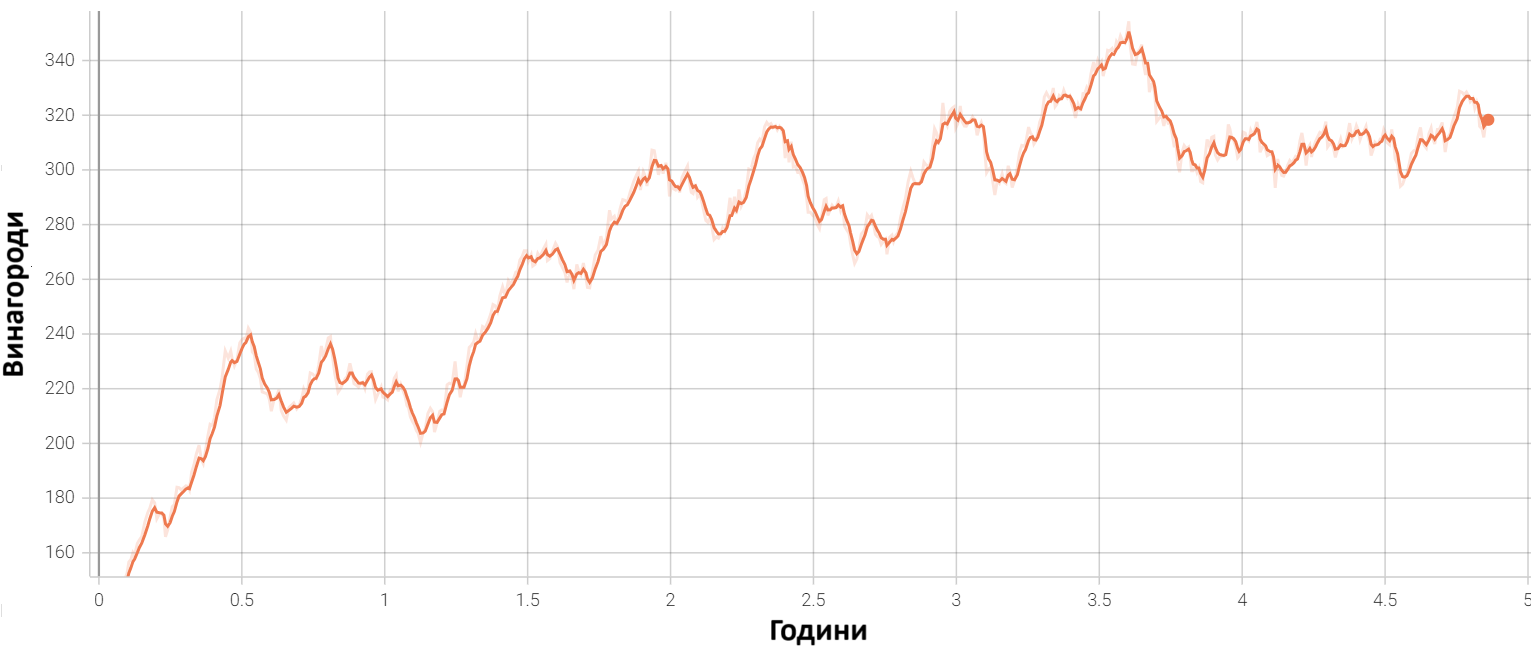
\includegraphics[scale = 0.65]{Pictures/DQN_REWARD.png}
    \caption{Графік зміни винагороди для DQN агента}
    \label{fig:DQN_REWARD}
\end{figure}

Аналізуючи рис \ref{fig:DQN_REWARD}, можна побачити, що модель DQN є 
здатною до ефективного навчання. Найбільші винагороди були отримані на 3 годині 
36 хвилині тренування(1.118 мільйоний крок), де максимальна винагорода становила 
354.4. Після цього моменту винагорода впала до 300.

Падіння винагороди після піку може бути пов'язане з кількома факторами:
\begin{itemize}
    \item \emph{Переобучення:} Модель могла почати переобучатися на специфічних станах, втрачаючи здатність узагальнювати стратегії на інші стани гри.
    \item \emph{Зміна стратегій:} Під час тренування агент міг перейти до нових стратегій, які тимчасово менш ефективні, але згодом можуть призвести до кращих результатів.
    \item \emph{Стохастичні зміни:} Природа алгоритмів підкріплювального навчання може призводити до випадкових коливань у винагородах, особливо під час експлоративних кроків.
\end{itemize}

Таким чином, незважаючи на тимчасове зниження винагороди, модель DQN демонструє 
здатність до ефективного навчання і покращення своїх стратегій в процесі тренування.
\subsection{PPO агент}
Модель Proximal Policy Optimization (PPO) була тренована на протязі 2 днів та виконала загалом 12 мільйонів кроків. 
Процес тренування був тривалим, але результативним, що дозволило моделі покращити свої стратегії та досягти високих результатів у грі.

\begin{figure}[H]
    \centering
    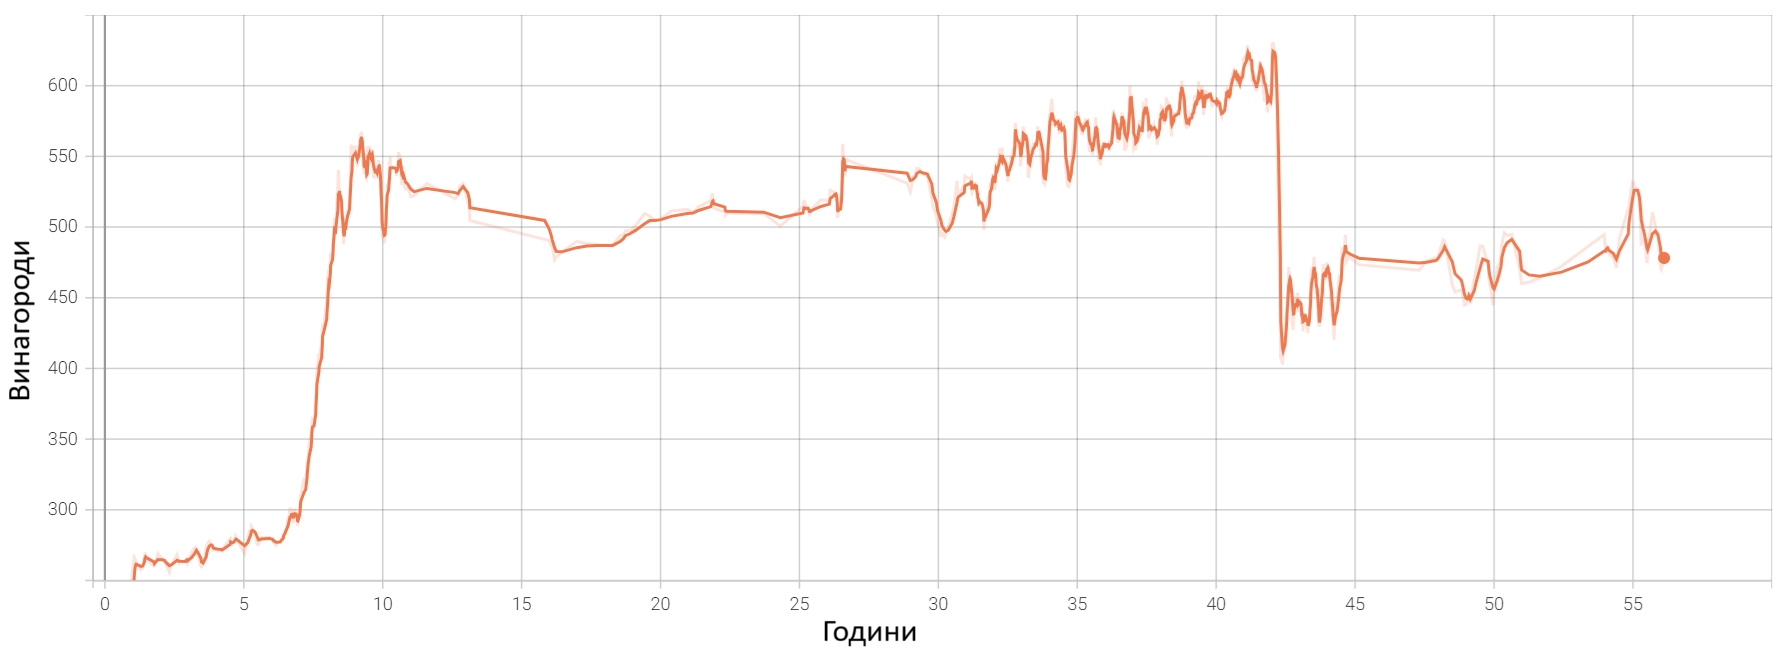
\includegraphics[scale = 0.55]{Pictures/PPO_REWARD.png}
    \caption{Графік зміни винагороди для PPO агента}
    \label{fig:PPO_REWARD}
\end{figure}

Аналізуючи рис \ref{fig:PPO_REWARD} моделі PPO, можна побачити 
наступні закономірності. До 7 години навчання середня винагорода моделі становила 250-300 очків. 
Однак, починаючи з 7 години (1.5 мільйона кроків) і до 8.5 години (2.3 мільйона кроків), модель 
неймовірно вистрілила, і її середнє значення винагороди становило 550 очків.

На 1 дні та 18 годині (9.28 мільйона кроків) навчання модель досягла свого максимального значення 
винагороди — 624 очки. Після цього винагорода моделі різко впала до 400 очків, і на останній годині 
тренування її винагорода становила 484 очки.

Падіння винагороди пов'язане зі зміною стратегії моделі. На своєму піку модель завжди 
переходила до правого краю екрану і, стоячи там, знищувала ворогів. Починаючи з 1 дня 18 години
 30 хвилин тренування (10 мільйонів кроків), модель змінила свою стратегію і почала навчатися тримати
  прямий контакт з ворогами. Ця нова стратегія могла бути менш ефективною в короткостроковій перспективі,
   що призвело до тимчасового зниження винагороди.
\subsection{A2C агент}
Модель A2C була піддана тренуванню на протязі 15.5 годин, що відповідає приблизно 14 мільйонам кроків. 
Під час тренування модель вдосконалювала свої стратегії та оцінювала цінність своїх дій, використовуючи 
ці дані для максимізації винагороди в грі.

\begin{figure}[H]
    \centering
    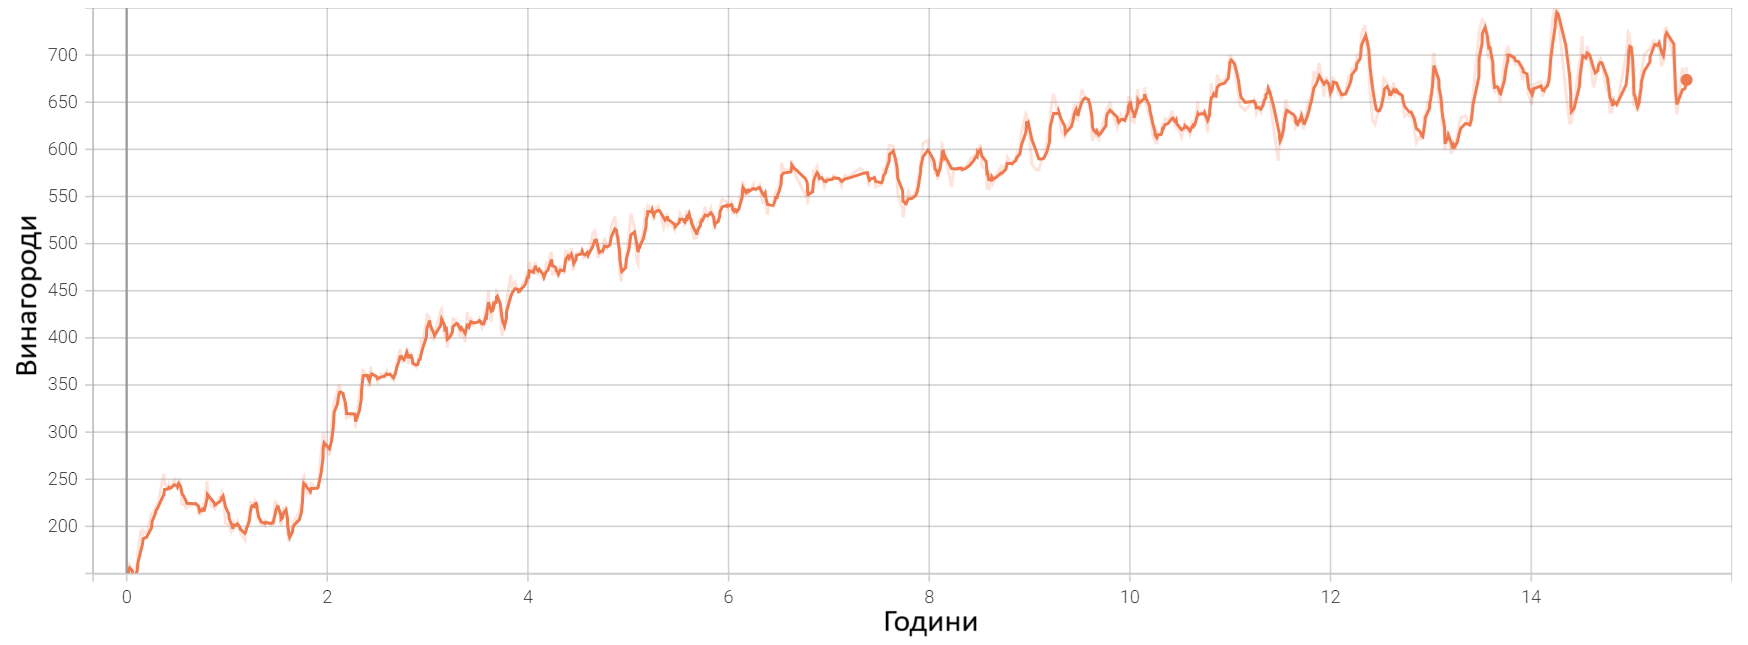
\includegraphics[scale = 0.55]{Pictures/A2C_REWARD.png}
    \caption{Графік зміни винагороди для A2C агента}
    \label{fig:A2C_REWARD}
\end{figure}

Під час аналізу рис \ref{fig:A2C_REWARD} моделі A2C ,було виявлено, що до 1 години 40 хвилин
 тренування модель демонструвала невисоку
  ефективність, з середньою винагородою близько 200 очок. Проте після цього періоду 
  спостерігалося помітне покращення її продуктивності.

Відзначається, що після першого періоду модель почала демонструвати стабільний логарифмічний зріст.
 Наприкінці п'ятої години тренування вона досягла значення 
 середньої винагороди у 531 очко, що є помітним покращенням порівняно з початковими 
 показниками. Це свідчить про здатність моделі до поступового та послідовного в\-дос\-коналення в 
процесі тренування, що дає підстави вважати, що вона може бути успішно навченою та
 досягнути високих результатів у майбутньому.\\
 \par Після аналізу графіків тренування для моделей DQN, PPO і A2C на грі Space Invaders можна 
 зробити наступний висновок: до п'ятої години тренування найкраще себе проявила модель A2C, після чого йшла модель DQN,
  а потім модель PPO. Проте після п'ятої години тренування модель PPO ней\-мовірно вистрілила,
 перегнавши DQN. У той час, модель A2C продовжувала 
 навчатися стабільно, залишаючись всі інші поделі позаду.

Аналізуючи ці дані, можна зробити висновок, що найкращою моделлю для гри Space Invaders є
 A2C. Це не дивно, оскільки модель A2C виявилася стабільною та ефективною протягом усього
  тренування, показавши найкращі результати до п'ятої години навчання та не втративши свою
   ефективність пізніше.
Отже, модель A2C виявилася кращою за інші моделі, такі як DQN та PPO, у грі Space Invaders.



